\section{Ponte Jakway Park}
\label{chap:jakway}

%Para elaborar este estudo de caso, utilizou-se a documentação disponibilizada pelo Departamento de Transporte do estado de Iowa, EUA e pelo e-mail cordialmente enviado pelo engenheiro Brian Keierbeler, com várias informações sobre o projeto da ponte Jakway Park.
%
%Na primeira seção, apresenta-se o processo de concepção do projeto e as motivações que levaram à escolha do CUAD como solução construtiva da ponte. Em seguida, estuda-se uma viga de seção retangular protendida feita com concreto convencional e comparando-a com uma feita em CUAD, calculando a força de protensão inicial exigida em cada uma. Neste trabalho, toma-se a liberdade de extrapolar as equações para cálculo de estruturas de concreto protendido da NBR 6118:2014 para uso em CUAD, já que a própria norma avisa que seus casos de uso são feitos para concretos com $ f_{ck} $ de até 90 MPa. É importante reforçar que ainda não existe normatização para o uso de CUAD em nenhum país, somente as recomendações de uso publicadas pela \cite{AFGC}\footnote{\textit{Association Française de Genie Civil}} e pela \cite{JSCE}\footnote{\textit{Japan Society of Civil Engineers}}, de modo que ainda é preciso desenvolver uma solução própria para cada caso.
%
%Também é importante lembrar que a visita ao empreendimento não foi possível, por conta de se encontrar nos Estados Unidos. Mesmo assim, foi possível observar as características e considerações utilizadas no projeto.
%
%\subsection{Características da locação da ponte Jakway Park}

Buchanan, no estado de Iowa, EUA é um município predominantemente rural. \citeonline{Keierleber_email} mostra que as pontes da cidade são muito antigas (muitas construídas entre 1870-1914) e já não são capazes de atender a demanda de veículos atuais. A  \autoref{acidente-1} e a \autoref{acidente-2} retratam acidentes ocorridos no município devido a esta deficiência.

\nomenclature[A]{MIT}{\textit{Massachusetts Institute of Technology}}
\nomenclature[A]{FHWA}{\textit{Federal Highway Administration}}

Como parte de um programa de pesquisa e financiamento através de um programa de construção de pontes inovadoras do governo dos EUA, o município decidiu trocar a velha ponte Jakway Park por uma ponte de CUAD seção $ \pi $, desenvolvida pelo Instituto de Tecnologia de Massachusetts (MIT) e pelo Laboratório Turner-Fairbank da Administração Federal de Rodovias (FHWA) \cite{Keierbeler_et_al}.

\begin{figure}[htb]
	\caption{\label{acidente-1}Acidente em ponte de madeira em Buchanan.}
	\begin{center}
		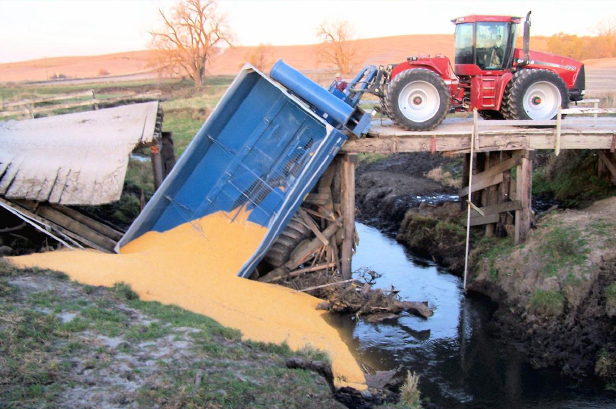
\includegraphics[max width=\textwidth]{acidente-1.png}
	\end{center}
	\fonte{\citeonline{Keierleber_email}}
\end{figure}

\begin{figure}[htb]
	\caption{\label{acidente-2}Acidente em Buchanan.}
	\begin{center}
		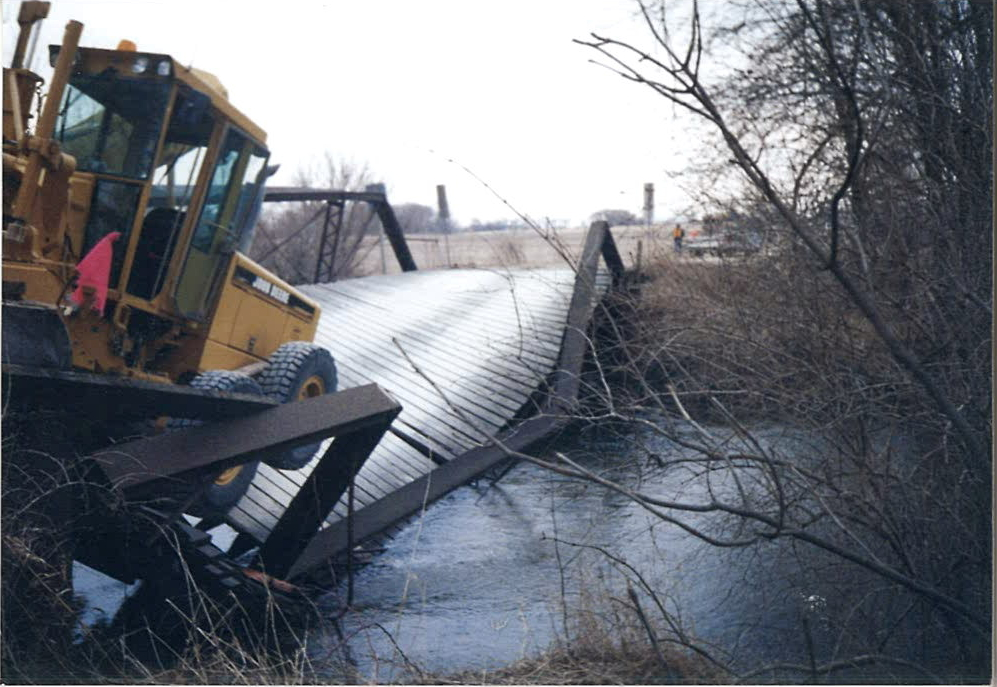
\includegraphics[max width=\textwidth]{acidente-2.jpg}
	\end{center}
	\fonte{\citeonline{Keierleber_email}}
\end{figure}

\subsection{Tabuleiro integral de seção \textpi}

O desenvolvimento da seção $ \pi $~começou a ser desenvolvido em 2003 no MIT. O projeto foi otimizado para aproveitar a superior resistência do CUAD para tensão, cisalhamento e compressão, usando a mínima área possível no corte transversal. A primeira geração da seção $ \pi $~(\autoref{secao-pi-1}) falhou nos testes de carregamento, levando os pesquisadores a iterar o projeto \cite[p.~4]{Rouse}. Entre os problemas encontrados, essa geração oferecia um tabuleiro de baixa rigidez, um preocupante comportamento de fissuração com cargas de serviço e problemas na distribuição da carga lateral entre as vigas adjacentes \apud[p.~1]{Graybeal}{Rouse}.

A segunda geração da seção $ \pi $~(\autoref{secao-pi-2}) resolveu os problemas da primeira, sem mudar drasticamente seu desenho, até por questões de economia e reaproveitamento das formas. Com o auxílio do Centro de Engenharia de Pontes (BEC\footnote{\textit{Bridge Engineering Center}}) da Universidade do Estado de Iowa (ISU\footnote{\textit{Iowa State University}}), foi criado um modelo de elementos finitos em 3D no programa ANSYS (\autoref{ansys}). Diversos modelos foram analisados para atender às mudanças necessárias e chegar ao desenho final da nova seção $ \pi $.

Na parte inferior das vigas foi instalado um diafragma metálico, adicionando algum grau de restrição rotacional global no fim das vigas \cite[p.~7]{Rouse}. Cada seção tem uma área de 0,555 m\textsuperscript{2} e um peso próprio de 13,63 kN/m \cite[p.~8]{Rouse}.

Para o dimensionamento das seções que foram utilizadas na construção, limitou-se a resistência a compressão a 148 MPa, por conta do método utilizado para misturar o concreto, o qual foi feito diretamente dentro do caminhão betoneira. Houve o temor que as fibras não se espalhassem da maneira correta, por isso ocorreu essa limitação \cite[p.~8]{Rouse}. A \autoref{valores-de-projeto} lista os dados levados em consideração para o projeto da ponte.

\begin{table}[htb]
	\IBGEtab{%
		\caption{Valores de projeto das propriedades materiais do CUAD.}
		\label{valores-de-projeto}
	}{%
	\begin{tabulary}{\linewidth}{CC}
		\toprule
		Propriedade                                   & Valor (MPa) \\
		\midrule \midrule
		Módulo de elasticidade à liberação            & 39,990 \\ \midrule 
		Módulo de elasticidade final	                 & 53,780 \\ \midrule 
		Resistência de compressão nominal à liberação & 86     \\ \midrule 
		Resistência de compressão nominal final	     & 148    \\ \midrule 
		Resistência nominal à tração final	         & 8,3    \\ \midrule 
		Perda de protensão permitida no escoamento	 & 51,7 (60\% de 86,16 MPa)   \\ \midrule
		Perda de protensão permitida no serviço       & 89   (60\% de 148,33 MPa)  \\ \midrule 
		Tensão de tração permitida no serviço	     & 5,8  (70\% de 8,30 MPa)    \\
		\bottomrule
	\end{tabulary}%
}{%
\fonte{\citeonline[p.~10]{Rouse}.}%
%\nota{Esta é uma nota, que diz que os dados são baseados na regressão linear.}
%\nota[Anotações]{Uma anotação adicional, que pode ser seguida de várias outras.}
}
\end{table}

\begin{figure}[htb]
	\caption{\label{secao-pi-1}Primeira geração da seção $ \pi $.}
	\begin{center}
		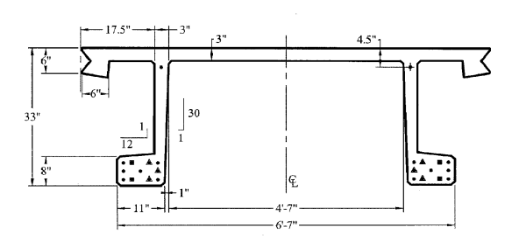
\includegraphics[max width=\textwidth]{secao-pi-1.png}
	\end{center}
	\fonte{\citeonline[p.~5]{Keierleber}}
\end{figure}

\begin{figure}[htb]
	\caption{\label{secao-pi-2}Segunda geração da seção $ \pi $.}
	\begin{center}
		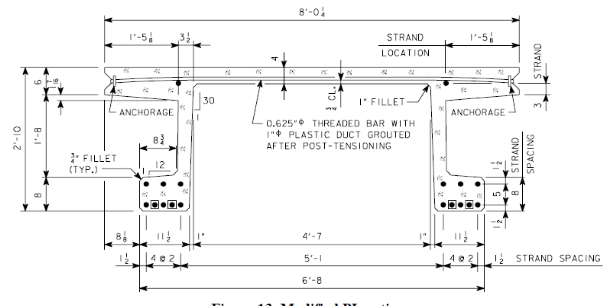
\includegraphics[max width=\textwidth]{secao-pi-2.png}
	\end{center}
	\fonte{\citeonline[p.~10]{Keierleber}}
\end{figure}

\begin{figure}[htb]
	\caption{\label{ansys}Modelo da seção $ \pi $~no ANSYS.}
	\begin{center}
		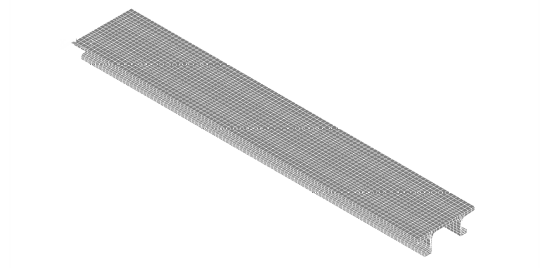
\includegraphics[max width=\textwidth]{ansys.png}
	\end{center}
	\fonte{\citeonline[p.~6]{Rouse}}
\end{figure}

\subsection{Construção}

A fornecedora do CUAD utilizado na obra (Lafarge) vende a mistura pronta do concreto. Para fazer o concreto, foi utilizado um caminhão betoneira, misturando o material cimentício, gelo e superplastificantes. Após a homegeinização do concreto, foram adicionadas as fibras de aço com uma peneira, afim de evitar seu agrupamento. Seguiu-se a transferência do CUAD para as formas \autoref{moldagem} e cura térmica a vapor a 90 \textsuperscript{\degree}C por 48 horas (\autoref{vapor}) \cite[p.~17]{Rouse}.

\nomenclature[S]{kN}{Quilonewton}

Em seguida, as peças foram transportadas para o local da construção. As seções adjacentes foram conectadas com barras de 25 mm, posicionadas a cada 45,7 cm e grauteadas (\autoref{corte}, \autoref{detalhe-juntas}  e \autoref{grauteamento}). Para a protensão, foram utilizados 22 cabos de 15 mm de diâmetro (\autoref{protensao}). Desses, 18 foram colocados no bulbo na base das vigas, e tensionados a uma força de 3407 kN. Os outros 4 foram colocados no tabuleiro e tensionados a 756 kN. Difragmas metálicos foram instalados na parte inferior das vigas (\autoref{detalhe-diafragma} e \autoref{foto-diafragma}).

Barras de 15 mm foram posicionadas na parte de baixo do tabuleiro, como reforço de flexão transversal. A instalação foi feita com o auxílio de gruas (\autoref{instalacao}).

A ponte Jakway Park (\autoref{jakway-park}) foi construída num intervalo de 52 dias, sendo inaugurada no dia 26 de novembro de 2008.

\begin{figure}[htb]
	\caption{\label{moldagem}Moldagem da seção $ \pi $.}
	\begin{center}
		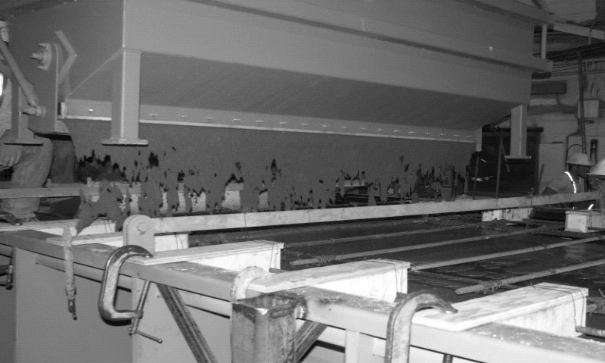
\includegraphics[max width=\textwidth]{moldagem.png}
	\end{center}
	\fonte{\citeonline[p.~17]{Rouse}}
\end{figure}

\begin{figure}[htb]
	\caption{\label{vapor}Cura térmica a vapor.}
	\begin{center}
		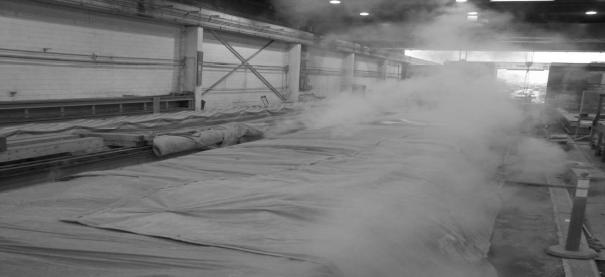
\includegraphics[max width=\textwidth]{vapor.png}
	\end{center}
	\fonte{\citeonline[p.~18]{Rouse}}
\end{figure}

\begin{figure}[htb]
	\caption{\label{corte}Vista em corte.}
	\begin{center}
		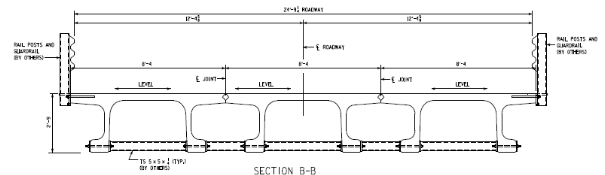
\includegraphics[max width=\textwidth]{corte.png}
	\end{center}
	\fonte{\apudonline[p.~16]{Kei}{Rouse}}
\end{figure}

\begin{figure}[htb]
	\caption{\label{detalhe-juntas}Detalhamento das juntas longitudinais da seção $ \pi $.}
	\begin{center}
		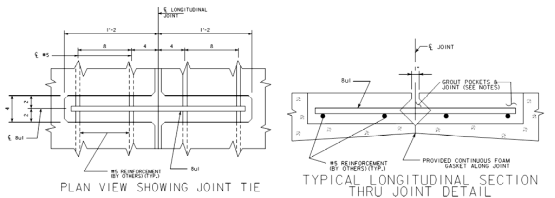
\includegraphics[max width=\textwidth]{detalhe-juntas.png}
	\end{center}
	\fonte{\citeonline[p.~15]{Rouse}}
\end{figure}

\begin{figure}[htb]
	\caption{\label{grauteamento}Grauteamento das juntas longitudinais.}
	\begin{center}
		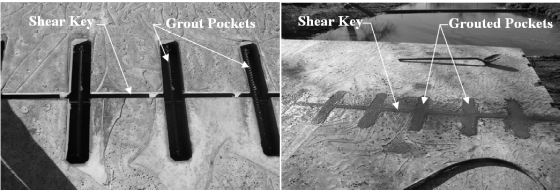
\includegraphics[max width=\textwidth]{grauteamento.png}
	\end{center}
	\fonte{\citeonline[p.~15]{Rouse}}
\end{figure}

\begin{figure}[htb]
	\caption{\label{protensao}Detalhe da protensão.}
	\begin{center}
		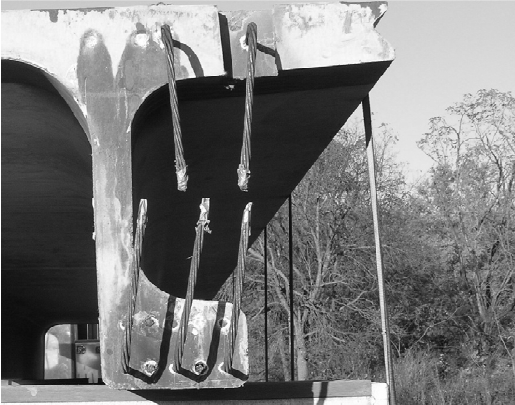
\includegraphics[max width=\textwidth]{protensao.png}
	\end{center}
	\fonte{\citeonline[p.~16]{Rouse}}
\end{figure}

% % %

\begin{figure}[htb]
	\caption{\label{detalhe-diafragma}Detalhamento do diafragma.}
	\begin{center}
		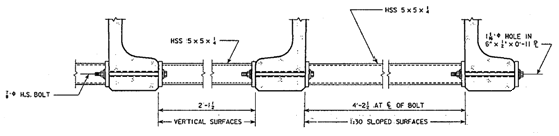
\includegraphics[max width=\textwidth]{detalhe-diafragma}
	\end{center}
	\fonte{\citeonline[p.~14]{Rouse}}
\end{figure}

\begin{figure}[htb]
	\caption{\label{foto-diafragma}Diafragma instalado entre as vigas de uma mesma seção e entre as vigas de seções adjacentes.}
	\begin{center}
		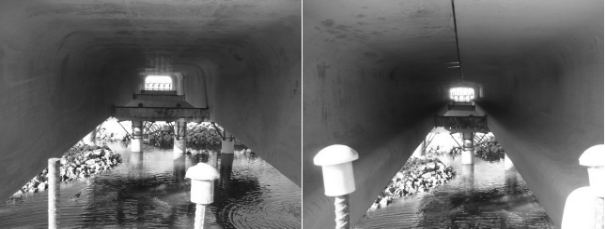
\includegraphics[max width=\textwidth]{foto-diafragma.png}
	\end{center}
	\fonte{\citeonline[p.~14]{Rouse}}
\end{figure}

\begin{figure}[htb]
	\caption{\label{instalacao}Instalação dos elementos estruturais.}
	\begin{center}
		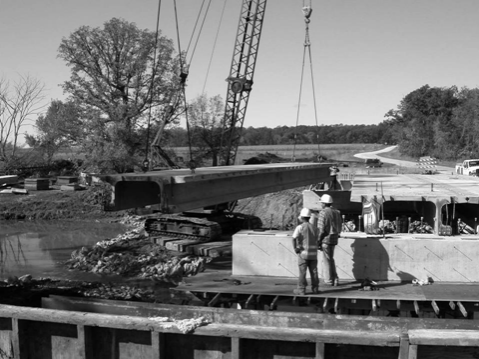
\includegraphics[max width=\textwidth]{instalacao.png}
	\end{center}
	\fonte{\citeonline[p.~18]{Rouse}}
\end{figure}

\begin{figure}[htb]
	\caption{\label{jakway-park}Ponte Jakway Park. Apenas o trecho do vão central é feito de CUAD.}
	\begin{center}
		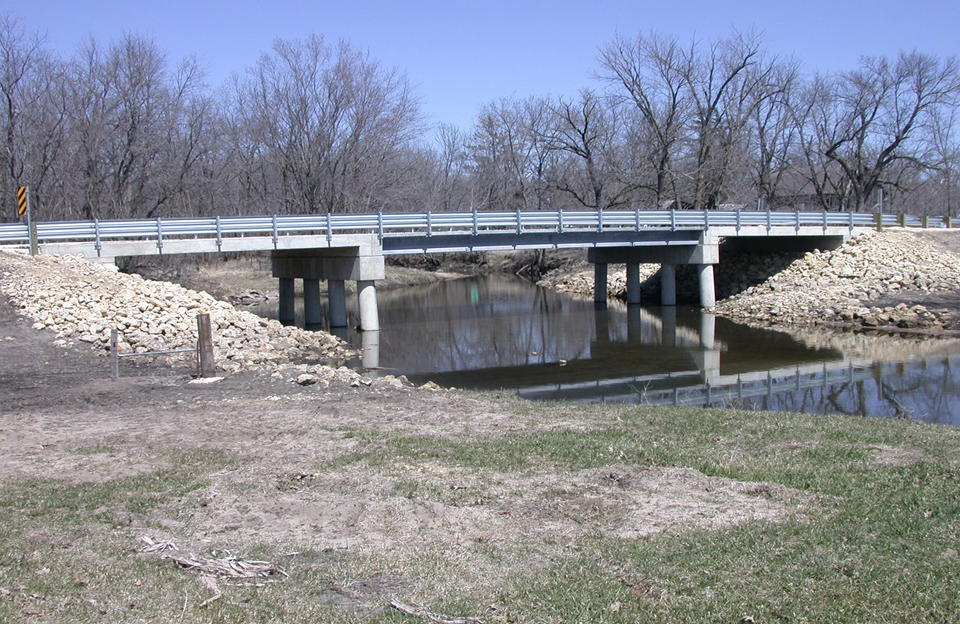
\includegraphics[max width=\textwidth]{jakway-park.png}
	\end{center}
	\fonte{\citeonline{Keierleber_email}}
\end{figure}